\documentclass[11pt]{article}

\usepackage[margin=2.5cm]{geometry}
\usepackage{amsmath,amssymb}
\usepackage{graphicx}
\usepackage{booktabs}
\usepackage{xcolor}
\usepackage{fancyhdr}
\usepackage{hyperref}
\usepackage{listings}
\usepackage{enumitem}
\usepackage{microtype}

\definecolor{headerblue}{RGB}{20,60,110}
\definecolor{codebg}{RGB}{245,245,245}

\lstset{
  backgroundcolor=\color{codebg},
  basicstyle=\ttfamily\small,
  breaklines=true,
  columns=fullflexible,
  frame=single,
  language=Java
}

\pagestyle{fancy}
\fancyhf{}
\renewcommand{\headrulewidth}{0.6pt}
\fancyhead[L]{\small AM5011 / Virtual Reality Engineering / Assignment 2}
\fancyfoot[C]{\small\thepage}

\title{\vspace{-1.5cm}\textcolor{headerblue}{\Large\textbf{AM5011 Virtual Reality Engineering}}\\[4pt]
\textcolor{headerblue}{\large Assignment 2: Dual Quaternions for VR Poses and Blending}}
\author{Your Name \quad | \quad Roll Number: XXXXXXX \quad | \quad Unity Version: 2022.3.52f1}
\date{}

\begin{document}
\maketitle
\thispagestyle{fancy}
\vspace{-1cm}

% =========================================================================
\section*{Part A --- Math and Representation}

\subsection*{1. Constructing the unit dual quaternion}

Let $q_r$ be a unit rotation quaternion ($\lVert q_r\rVert = 1$) and let
$t = (t_x, t_y, t_z)$ be a translation vector, embedded as the pure
quaternion $T = (t_x, t_y, t_z, 0)$.

A pure rotation has zero dual part:
\[
\hat{R} = q_r + \epsilon \cdot 0.
\]
A pure translation is represented as
\[
\hat{T} = 1 + \tfrac{1}{2}\epsilon T.
\]
Applying the rotation first and the translation second corresponds to
$\hat{q} = \hat{T}\hat{R}$:
\[
\hat{q} = \left(1 + \tfrac{1}{2}\epsilon T\right)(q_r + 0\cdot\epsilon)
        = q_r + \epsilon\left(\tfrac{1}{2} T q_r\right).
\]

\begin{quote}
\textbf{Derived unit dual quaternion:}
\[
\hat{q} = q_r + \epsilon q_d, \qquad q_d = \tfrac{1}{2} T q_r.
\]
\end{quote}

Since $\lVert q_r \rVert = 1$ and $q_r \cdot q_d = \operatorname{Re}(q_d q_r^{*}) =
\operatorname{Re}(\tfrac12 T) = 0$, $\hat{q}$ satisfies both unit dual
quaternion constraints and validly encodes the 6-DOF pose $(R, t)$.

\subsection*{2. Recovering $R$ and $t$ from $\hat{q}$}

The real part directly gives the rotation, renormalized to remove drift:
\[
R = \frac{q_r}{\lVert q_r \rVert}.
\]

To recover the translation, start from $q_d = \tfrac12 T q_r$ and
right-multiply by $q_r^{-1}$. Since $q_r$ is unit, $q_r^{-1} = q_r^{*}$:
\[
2 q_d q_r^{*} = T (q_r q_r^{*}) = T
\qquad\Longrightarrow\qquad
T = 2 q_d q_r^{*}.
\]
The vector part of the resulting pure quaternion $T$ is the recovered
translation $t = (T_x, T_y, T_z)$; its scalar component is zero up to
floating-point error.

\subsection*{3. Why dual quaternions for VR blending?}

Natural VR motions --- a controller swinging through an arc, a shoulder-elbow-wrist
chain articulating --- combine rotation and translation along a single curved
path, not two independent straight-line channels. Blending position and
rotation separately (\texttt{Vector3.Lerp} + \texttt{Quaternion.Slerp}) forces
the object along a flat chord between the two endpoints while the orientation
turns independently, which is exactly the decoupling that produces
"candy-wrapper" mesh collapse in skinning and visibly unnatural sliding motion
for a single rigid object. A dual quaternion blends translation and rotation
as one coupled 6-DOF quantity, so the interpolated pose follows the true
spatial screw motion between the two poses (Chasles' theorem) instead of an
arbitrary decoupled path.

\subsection*{Composition (used by \texttt{DualQuaternion.Multiply})}

\[
\hat{q}_a \hat{q}_b = (q_{r,a} q_{r,b}) + \epsilon (q_{r,a} q_{d,b} + q_{d,a} q_{r,b}).
\]
\texttt{Multiply(a, b)} applies $b$ first, then $a$: $R = R_a R_b$ and
$t = R_a t_b + t_a$, matching Unity's own quaternion/transform composition
order.

% =========================================================================
\section*{Part B --- Implementation (Unity C\#)}

\texttt{Assets/Scripts/DualQuaternion.cs} implements the struct exactly as
specified:

\begin{itemize}
  \item \textbf{Fields:} \texttt{Quaternion r} (real part), \texttt{Quaternion d} (dual part).
  \item \texttt{FromPose(rotation, translation)} --- builds $\hat q = q_r + \epsilon(\tfrac12 T q_r)$.
  \item \texttt{ToPose(out rotation, out translation)} --- extracts $R = q_r/\lVert q_r\rVert$ and $t = 2 q_d q_r^{*}$.
  \item \texttt{Multiply(a, b)} --- rigid composition as derived above.
  \item \texttt{Slerp(a, b, u)} --- dual quaternion linear blending (DLB): shortest-path
    sign alignment on the real part, \texttt{Quaternion.Slerp} on $q_r$, a
    \emph{componentwise} \texttt{Mathf.Lerp} on $q_d$, then re-normalization.
  \item \texttt{Normalized()} / \texttt{Conjugate()} --- enforce $\lVert q_r\rVert = 1$,
    $q_r \cdot q_d = 0$, and provide the dual quaternion conjugate.
\end{itemize}

\paragraph{Two implementation details that matter.} Unity's \texttt{Quaternion}
type has no operators for quaternion addition or scalar multiplication between
two quaternions, so every dual-part operation is written out componentwise
rather than relying on \texttt{Quaternion} arithmetic. Second, the dual part of
the identity pose is the \emph{zero} quaternion $(0,0,0,0)$, not
\texttt{Quaternion.identity} (which is $(0,0,0,1)$) --- using the latter would
silently encode a phantom translation. Likewise, \texttt{Slerp} blends the dual
part with \texttt{Mathf.Lerp} component-by-component rather than
\texttt{Quaternion.Lerp}, which renormalizes its result to a unit quaternion
and would corrupt the (generally non-unit) dual part.

\subsection*{Demo scene}

\texttt{Assets/Scripts/Editor/SceneSetupHelper.cs} adds an editor menu item,
\textbf{AM5011 $\to$ Build Full Demo Scene}, that constructs the scene
programmatically (since a hand-authored \texttt{.unity} file cannot be
produced outside the Unity Editor reliably):

\begin{itemize}
  \item \texttt{PoseA} (red) and \texttt{PoseB} (green) as fixed pose anchors.
  \item \texttt{InterpolatedPose} (cyan), driven by\\
    \texttt{DualQuaternionPoseDemo.cs} using \texttt{DualQuaternion.Slerp}.
  \item \texttt{DecoupledPose} (magenta), driven by plain \texttt{Vector3.Lerp}
    and \texttt{Quaternion.Slerp} for the Part C comparison.
  \item A UI \texttt{Slider} (0--1) bound to the interpolation parameter $u$, plus
    a \texttt{TrailRenderer} on each pointer to visualize the swept path.
\end{itemize}

\texttt{Assets/Scripts/DualQuaternionMathTests.cs} is a Play-mode sanity check:
it verifies the \texttt{FromPose}/\texttt{ToPose} roundtrip, that
\texttt{Slerp} exactly recovers both endpoints at $u=0,1$, that the blended
pose stays a valid unit dual quaternion at $u=0.5$, and that \texttt{Multiply}
composes two poses the same way Unity's own transform chaining does.

% =========================================================================
\section*{Part C --- Mini-Experiment: Controller Interpolation}

\textbf{Setup.} PoseA is placed at $(-2, 0, 0)$~m with identity rotation;
PoseB is placed at $(2, 0, 0)$~m rotated $120^\circ$ about $+Z$. Both methods
interpolate between the identical pair of endpoints:
\begin{enumerate}[nosep]
  \item \textbf{Separate:} \texttt{Vector3.Lerp} on position, \texttt{Quaternion.Slerp} on rotation.
  \item \textbf{Dual-quaternion Slerp (DLB):} \texttt{DualQuaternion.Slerp(dqA, dqB, u)}.
\end{enumerate}

\begin{figure}[h]
  \centering
  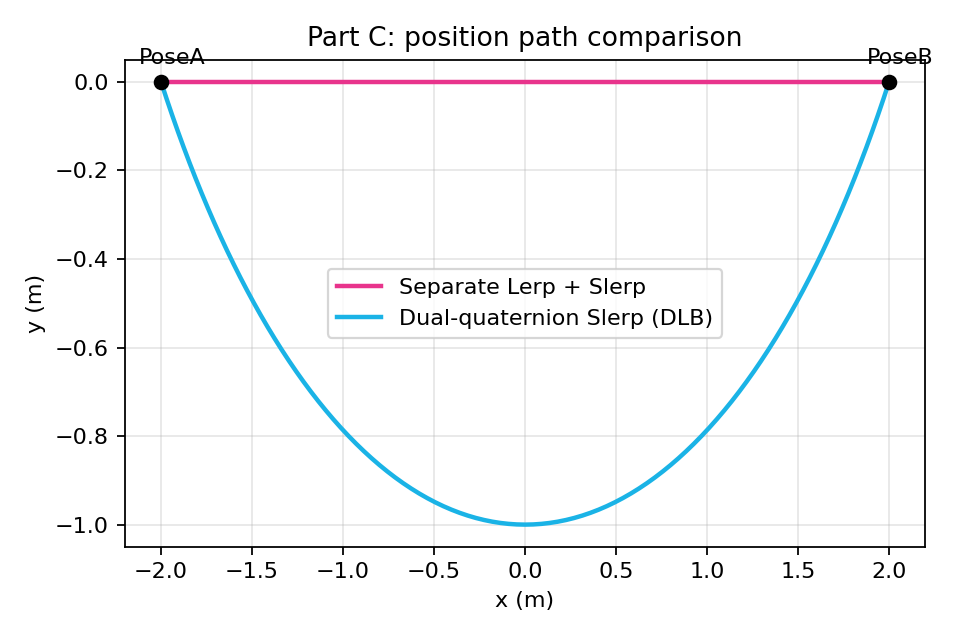
\includegraphics[width=0.72\textwidth]{figures/trajectory_comparison.png}
  \caption{Computed position path for both methods, sampled at 101 values of $u \in [0,1]$
  (\texttt{tools/dualquat\_sim.py}, a numeric replica of \texttt{DualQuaternion.cs}).}
\end{figure}

\begin{table}[h]
\centering
\begin{tabular}{@{}ccccc@{}}
\toprule
$u$ & DLB $x$ (m) & DLB $y$ (m) & DLB angle & Separate angle \\
\midrule
0.00 & $-2.000$ & $0.000$  & $0.00^\circ$   & $0.00^\circ$   \\
0.25 & $-1.095$ & $-0.742$ & $30.00^\circ$  & $30.00^\circ$  \\
0.50 & $0.000$  & $-1.000$ & $60.00^\circ$  & $60.00^\circ$  \\
0.75 & $1.095$  & $-0.742$ & $90.00^\circ$  & $90.00^\circ$  \\
1.00 & $2.000$  & $0.000$  & $120.00^\circ$ & $120.00^\circ$ \\
\bottomrule
\end{tabular}
\caption{Position and orientation at five sample values of $u$.}
\end{table}

\subsection*{Observations}

\begin{itemize}
\raggedright
  \item \textbf{Curved vs.\ straight path:} the separate method's position
    follows the straight chord $y=0$ between the anchors; DLB's position
    follows a curved arc dipping to $y = -1.0$~m at $u=0.5$. Coupling rotation
    into the translation term ($q_d = \tfrac12 T q_r$) is exactly what bends
    the path.
  \item \textbf{Orientation profile is identical here:} both methods compute
    the rotation as \texttt{Quaternion.Slerp} of the same endpoint
    quaternions, so the angle-vs-$u$ curve matches exactly in this
    experiment. The two methods diverge only in \emph{where the translation
    goes}, not in the rotation timing --- for a genuine screw motion (dual
    quaternion) this coupling is precisely what decoupled Lerp + Slerp
    cannot express.
  \item \textbf{Naturalness for VR:} the curved DLB path is consistent with a
    joint (shoulder, elbow, wrist) sweeping a controller through an arc; the
    straight-chord path of separate interpolation looks mechanical and
    unnatural for a rotating hand or tool, since it is only correct when
    translation and rotation are physically independent.
  \item \textbf{Rigidity is preserved either way:} because \texttt{Normalized()}
    is applied after every blend, DLB stays on the unit dual-quaternion
    manifold throughout $u \in [0,1]$; there is no collapse or scale drift at
    the midpoint.
  \item \textbf{Caveat:} this simple DLB (linear blend + re-normalize) is an
    approximation to true constant-speed ScLERP; for large rotation angles or
    widely separated anchors the coupling is even more pronounced, which is
    the effect exploited for avatar-skinning artifact reduction (Kavan et al., 2008).
\end{itemize}

% =========================================================================
\section*{Deliverables}
\begin{itemize}[nosep]
\raggedright
  \item \path{Assets/Scripts/DualQuaternion.cs}, \path{DualQuaternionPoseDemo.cs},
    \path{Editor/SceneSetupHelper.cs}, \path{DualQuaternionMathTests.cs}.
  \item \path{tools/dualquat_sim.py} --- numeric verification and Part C figure and table generator.
  \item This report (\path{report/main.tex}).
\end{itemize}

\end{document}
